% File example.tex
% Contact: simonnet@ecole.ensicaen.fr
%
% version 1.0 (July 24, 2009)
% version 1.1 (September 3, 2009)
% add using of the optional command: \secondauthoraddr

\documentclass[10pt]{article}

% File icdp2009.sty
% Preamble that you have to include to use the template  

% July 24, 2009
% Contact: simonnet@ecole.ensicaen.fr


\usepackage[a4paper,textwidth=18cm,textheight=24cm,top=2.85cm, bottom=2.85cm, left=1.5cm, right=1.5cm]{geometry}

\usepackage{includes/icdp2009}

% left justified caption
\makeatletter
\long\def\@makecaption#1#2{%
\vskip\abovecaptionskip
\sbox\@tempboxa{#1. #2}%
\ifdim \wd\@tempboxa >\hsize
#1. #2\par
\else
\global \@minipagefalse
\hb@xt@\hsize{\box\@tempboxa\hfil}%
\fi
\vskip\belowcaptionskip}
\makeatother




%other package

% vectorial font
\usepackage{lmodern}

\usepackage{graphicx}
\usepackage{times}

\usepackage{textcomp}
\usepackage[justification=centering]{caption}
\usepackage{subcaption}
\usepackage{enumitem}

\begin{document}
\noindent

% This should produce references in the order they appear
\bibliographystyle{ieeetr}

\title{Automatically landmarks prediction on Beetle's pronotum}
%\title{An improvement on estimated landmarks of Beetle's pronotum}

\authorname{Van Linh Le$^{1,3}$, Marie Beurton-Aimar$^{1}$, Akka Zemmari$^1$, Nicolas Parisey$^2$}
\authoraddr{$^1$LaBRI - CNRS 5800 Bordeaux University, France, van-linh.le/beurton/zemmari@labri.fr}

%optional
\secondauthoraddr{$^2$IGEPP - INRA 1349, France, nparisey@rennes.inra.fr }
\thirdauthoraddr{$^3$ITDLU - Dalat University, Vietnam, linhlv@dlu.edu.vn}


\maketitle

\keywords
Landmarks, convolutional neural networks, fine-tuning, recogntion, procrustes.

\abstract
%Morphometry landmakrs were used in many biological application. Mostly, the landmarks are defined manually or semi-automatic by applying the image processing techniques.
In recent years, deep learning is known as a good solution for the difficult problems in computer vision. It appears in many fields such as classification, recognition, face detection. In this paper, we propose a scenario to predict the landmarks on 2D images, specify beetle's head images. The proposed method includes two stages: firstly, the landmarks are estimated by applying convolutional neural network; then, the estimated landmarks are improved to increase the accuracy. The method experimented on a set of 293 images. The accuracy of the method is evaluated by calculating the distance in pixels between the coordinates of the predicted landmarks and manual landmarks which were provided by the biologists.

\section{Introduction}
Morphometry landmark (or point of interest) is an important feature in many biological investigations. It was usually used to analyze the forms of whole biological organs or organisms. The analysis is mainly based on the coordinates of the landmarks. The collecting of enough the number of landmarks can help the biologists make a good estimate about organisms. Depending on the problem, the number of landmarks may be more or less; besides, the location of landmarks can be located on the shape (border) or inside the object, \textit{for examples,} the landmarks on Drosophila wings have stayed on the veins of the wings but the landmarks on human ear can be located at the ear hole or inside. Recently, the landmarks were set manually by the biologists. This work is time-consuming and difficult to reproduce. Therefore, a method that proposes automatically the coordinates of landmarks could be a concern. 

Based on the characteristics of digital images acquired for morphological studies, the images can be divided into two groups: the images where they are easy to segment the objects of interest, called \textit{segment-able images}; and the images that we can go in tight when segment the objects, called \textit{un-segment-able images}. For that reason, the methods that used to identify the landmarks automatically may be divided into two groups too. For segment-able images, identification of landmarks on the shape can be finished by applying the image processing techniques such as HOG\cite{palaniswamy2010automatic}, SIFT\cite{lowe2004distinctive}, .... But for un-segment-able images, defining the landmarks become a challenge and the image processing techniques seem to be inappropriate. This article introduces a scenario for automatic detection of the landmarks on biological images, specific beetle's pronotum images (Fig. \ref{figpronotum}). The method includes 2 stages: 1) The initially predicted landmarks are given by a convolutional neural network (CNN) \cite{lecun2010convolutional}. The main idea of this stage is design and train a CNN with a set of images and their manual landmarks. The dataset includes $293$ pronotum images and their manual landmarks which have been provided by the biologists. The images are presented in two dimensions and RGB color. After training, the trained network will be able to detect the initially predicted landmarks on the pronotum images; 2) The predicted landmarks which located in the shape of pronotum will be refined the location to increase the accuracy of coordinates. This stage is done by applying a Procrustes analysis\cite{gower1975generalized}. For each manual landmark, a model is generated as a specific. Then, it is used to refine the corresponding predicted landmarks.

\begin{figure}[htbp]
\centering
	\centerline{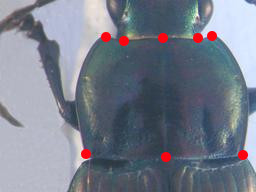
\includegraphics[scale=0.75]{images/pronotum}}
	\caption{An example of pronotum images and its manual landmarks}
	\label{figpronotum}
\end{figure}

In the next section, we present related works in domain automatically estimation landmarks on 2D images. In section 3, we present an overview about the stage that predict the initial automatically landmarks by applying CNN. It shows also the training process and experiment stage. The procedure that apply to improve the coordinates of predicted landmarks by CNN will be presented in section 4. In the last section, we have some conclusion based on the experiments and analysing the results.

\section{Related works}
Landmarks or points of interest are one of the important characteristics in geometric morphometrics. Landmark studies have traditionally analyzed on 2D images. Depending on which situation was stayed (segment-able or un-segment-able images), setting landmarks must apply the different methods.

When segmentation can be applied, Lowe et al. \cite{lowe2004distinctive} have proposed a method to identify the key points in the 2D image. From the detected key points, the method is able to match two images. Palaniswamy et al. \cite{palaniswamy2010automatic} have applied probabilistic Hough Transform to automatically estimate the landmarks in images of Drosophila wings. Adrien et al. \cite{le2017maelab} have extended Palaniswamy's method to detect landmarks automatically on beetles mandibles. Unfortunately, this method can not be applied to other parts of beetle that the segmentation has too many noises, such as pronotum images.

Recently years, machine learning is developing rapidly, specifically deep learning (CNN). It exists in most of the fields, especially in computer vision. We can finish a lot of difficult tasks with a deep convolution neural network such as classification \cite{krizhevsky2012imagenet, ciregan2012multi}, image recognition \cite{szegedy2015going, farabet2013learning, li2015convolutional}, speech recognition \cite{mikolov2011strategies, hinton2012deep} and language translation \cite{jean2014using, sutskever2014sequence}. Using CNN to determine landmarks on 2D images will produce good results and it may be a good solution for the un-segment-able images. Yi Sun et al. \cite{sun2013deep} have proposed a cascaded convolutional network to predict the key points on the human face. Zhang et al. \cite{zhang2014facial} optimizes facial landmarks detection with a set of related tasks such as head pose estimation, age estimation, .... Cintas et al. \cite{cintas2016automatic} have introduced a network to predict the landmarks on human ear images. In the same context, we have applied CNN to predict the landmarks on pronotum images. The predicted landmarks then refined to increase the accuracy of coordinates.

\section{Automatic landmarks by using CNN}
Deep learning presents a learning method with multiple levels of representation of connected layers (convolutional neural network). Data representation is transformed from a lower level to a higher level with many complex functions can be learned via backpropagation. In this section, we will present a CNN that we used to predict the landmarks on pronotum images. Besides, the techniques that applied to preprocess data before using for training the network.
\subsection{Network architecture}
Like the other networks \cite{lecun2010convolutional, li2015convolutional, cintas2016automatic}, the proposed network consists of several common layers with different learnable parameters (Fig.\ref{cnnnetwork}). It receives an input of $1 \times 256 \times 192$ to train, validate, and test. The network consists of three repeated-structure of a convolutional layer followed by a maximum pooling layer and a dropout layer. The depth
of convolutional layers increases from $32$, $64$, and $128$ with
different size of the filter kernel: $3 \times 3$, $2 \times 2$, and $2 \times 2$.
All the kernels of pooling layers have the same size of $2 \times 2$. The probability values used for dropout layers are $0.1, 0.2,$ and $0.3$.
At the end, three full connected layers have been added to the
network. The outputs of the full connected layers are $1000$, $1000$,
and $16$, respectively. The output of the last full-connected
layer corresponds to 8 landmarks (x and y coordinates) which
we would like to predict. Additional, to have a better control of overfitting, another dropout layer with a probability of $0.5$ is inserted between the first two full connected layers \cite{srivastava2014dropout}.

\begin{figure}[htbp]
\centering
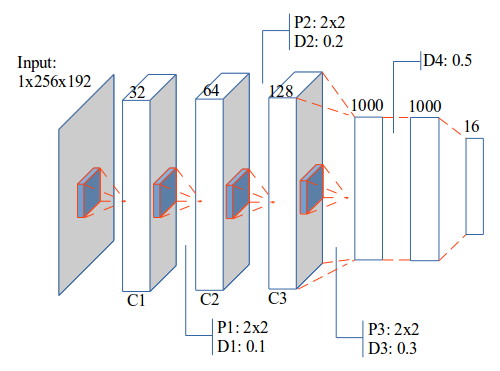
\includegraphics[scale=0.5]{images/architecture3}
\caption{The architecture of the proposed convolutional neural network} 
\label{cnnnetwork}
\end{figure}

During training, the values of learnable parameters have been updated to increase the accuracy of the network by applying gradient descent in backward phase. Therefore, the network is designed with a small sharing learning rate and momentum. Their values are updated over training time to fit with the number of epochs. The implementation of the network is done on Lasagne framework \cite{lasagne} which allows computing on GPU. The network has been trained on NVIDIA TITAN X cards.

\subsection{Data processing}
The dataset includes $293$ pronotum images of beetles. All images are taken with the same camera in the same condition with a resolution of $3264 \times 2448$. Each image has been set $8$ manual landmarks by biologists (Fig. \ref{figpronotum}). The dataset was split into two subsets: training (and validation) set contains $260$ images and testing set includes $33$ images. In most of CNNs \cite{lecun2010convolutional, sun2013deep,  krizhevsky2012imagenet, cintas2016automatic}, the size of the input was limited to $256$ pixels. In our case, the resolution of input image seems that too large and it becomes a difficulty for the network. So, the images are down-sampling to a new resolution $256 \times 192$ before training and testing. Of course, the coordinates of manual landmarks are also scaled to fit with the new resolution of images.

Besides the size of the input, the number of images is also a challenge when applying CNN. Normally, training a CNN with a large dataset will give us the result better than when we training CNN on a small dataset. Moreover, working with a small dataset, we can meet a popular problem, \textit{overfitting}. So, we need to enlarge the size of the dataset instead of $293$. In image processing, we usually apply transform procedures (translation, rotation) to generate a new image but in fact, when we compute the value of the pixels, it does not change while CNN computes the values of the pixels. Therefore, we have applied two other procedures to increase the number of images in the dataset. To address this problem, we have applied two procedures to enlarge the size of the dataset.

The first procedure was applied to change the value of each
channel in the original image. According to this, a constant is
added to a channel of RGB image and for each time, we just
change the value of one of three channels. For example, from
an original RGB image, if we add a constant c = 10 to the
red channel, we will obtain a new image with the values at
red channel by greater than the red channel of original image
a value of 10. By this way, we can generate three new RGB
images from a RGB image.

The second procedure is splitting the channels of RGB
images. It means that we separate the channels of RGB into
three gray-scale images. This work seems promising because
the network works on single-channel images. At the end, we
can generate six versions from an image, the total number of
images used to train and validate is $260 \times 7 = 1820$ images
(six versions and original image).
%\begin{table}[h]
%\begin{center}
%\begin{tabular}{c}
%nn!1 \\
%2 \\
%31 \\
%6 \\
%\end{tabular}
%\end{center}
%\caption{\label{tab1}This is an example of a table caption.}
%\end{table}
%\begin{equation}
%	    PA + A'P - PBR^{-1}B'P + Q  =  0 \enspace.
%\end{equation}

\subsection{Training and experiments}
\label{straining}
The network was trained on a dataset of $1820$ images. The number of images that
used for training and validation is splitted randomly by a ratio
(training: $80\%$, validation: $20\%$) that has been set during the
network setup. During the training, the network learned the information through a pair of \textit{(image, landmarks)} in training set. At the test phase, the image without landmarks was given to the trained network and the predicted landmarks will be given at the output. In practical of CNN, convergence is
usually faster if the average of each input variable over the
training set is close to zero. Moreover, when the input is set
closed with zero, it will be more suitable with the sigmoid
activation function \cite{lecun2012efficient}. According to \cite{lecun2012efficient}, the brightness of
the image is normalized to $[0; 1]$, instead of $[0; 255]$ and the
coordinates of the landmarks are normalized to $[-1; 1]$, instead
of $[0; 256]$ and $[0; 192]$ before giving to the network.

The training was finished in $5000$ epochs\footnote{An epoch is a single pass through the full training set}. The learning rate was initialized at $0.03$ and stopped at $0.00001$, while the momentum was updated from $0.9$ to $0.9999$. 
Because landmarks prediction can be seen as a regression problem in deep learning. Therefore, the root mean square error (RMSE) was used as a quality metric to evaluate the result and compute the losses of the proposed architecture.

Fig. \ref{cnnlosses} shows the training error and the validation error during training time. The blue curve presents RMSE error on training data. The green curve presents the validation error. Clearly, the losses are very different from the beginning. But, the difference is narrowed when the epoch increase.

\begin{figure}[htbp]
\centering
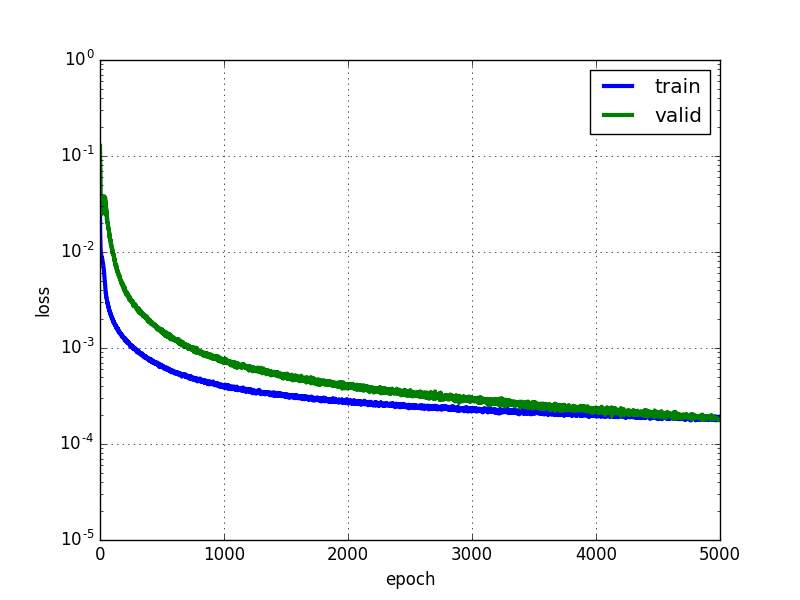
\includegraphics[scale=0.417]{images/losses}
\caption{The loss curves during training of proposed network} 
\label{cnnlosses}
\end{figure}

Besides the losses during training, the accuracy on coordinates of predicted landmarks of the test images is also considered. Firstly, the trained model was used to predict the landmarks on all images in the test set. Then, the distance (in pixels) between manual and corresponding landmarks in each image was calculated as the error distance. Finally, the error distance per landmark was calculated for all test images. Table.\ref{tabledistance} shows the average error distance given on each landmark. With the size of the images is $256 \times 192$, if we accept an error around $3\%$ of the image size ($ \sim3.5$ pixels), the error distances are acceptable.

\begin{table}[htbp]
\centering
\begin{tabular}{|c|p{1.5cm}|}
\hline
\textbf{$\#$Landmark} & \textbf{Distance} \\ \hline
1 & 4.002  \\ \hline
2 & 4.4831 \\ \hline
3 & 4.2959 \\ \hline
4 & 4.3865 \\ \hline
5 & 4.2925 \\ \hline
6 & 5.3631 \\ \hline
7 & 4.636 \\ \hline
8 & 4.9363 \\ \hline
\end{tabular}
\caption{The average error distance per landmark}
\label{tabledistance}
\end{table}
Fig.\ref{figrsexample} shows the predicted landmarks on two test images. When we consider the accuracy of predicted landmarks by calculating the distance between manual and corresponding predicted landmarks, the accuracy on coordinates of predicted landmarks on Fig.\ref{figsub1} is $99\%$ and the propotion on Fig.\ref{figsub2} is $80\%$.

\begin{figure}[htbp]
    \centering
    \begin{subfigure}[t]{0.25\textwidth}
        \centering
        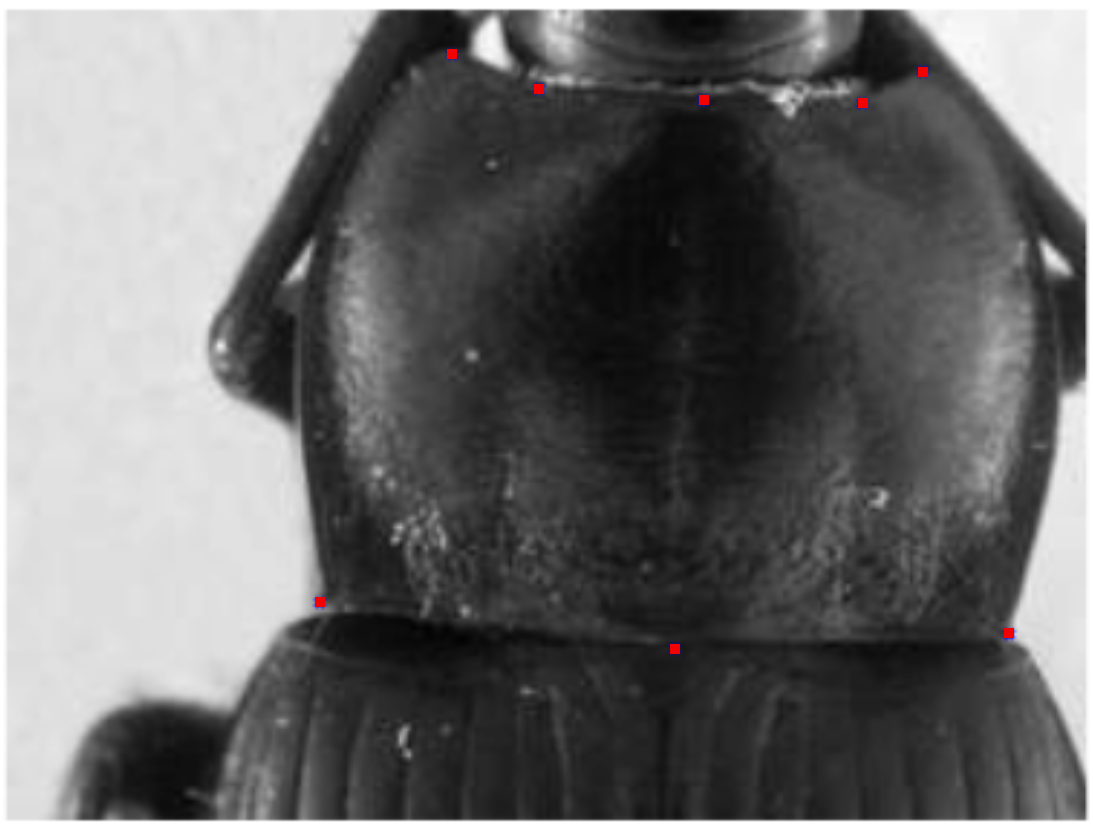
\includegraphics[height=1.2in]{images/plandmark}
        \caption{Image with well-predicted landmarks}
        \label{figsub1}
    \end{subfigure}%
    ~ 
    \begin{subfigure}[t]{0.25\textwidth}
        \centering
        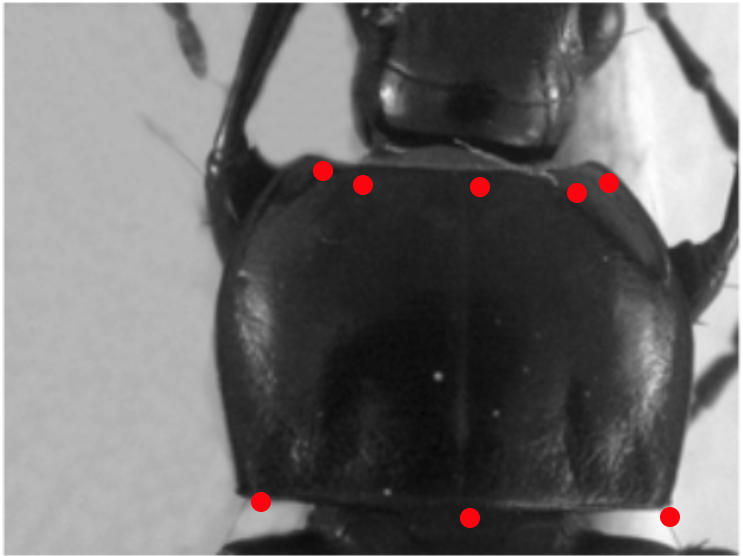
\includegraphics[height=1.2in]{images/plandmark2}
        \caption{Image with inaccuracy landmarks}
        \label{figsub2}
    \end{subfigure}
    \caption{The predicted landmarks on an image in test set.\\
    		 The read points present for the predicted landmarks}\
    \label{figrsexample}
\end{figure}

To have a better evaluation of the predicted landmarks, we have applied the standard deviation \cite{bland1996statistics} to quantify the dispersion of a set of distances. In this case, a predicted landmark is considered as acceptable if its error distance to the corresponding manual landmark is less than the average error (per landmark) plus standard deviation value. Fig. \ref{figchart} shows the ratio of acceptable per landmark. Most of landmarks have been predicted with the accuracy grater than \textbf{$70\%$}. In which, the lowest and highest prediction accuracies are \textbf{$66.67\%$} and \textbf{$87.88\%$}, respectively.

\begin{figure}[htbp]
	\centerline{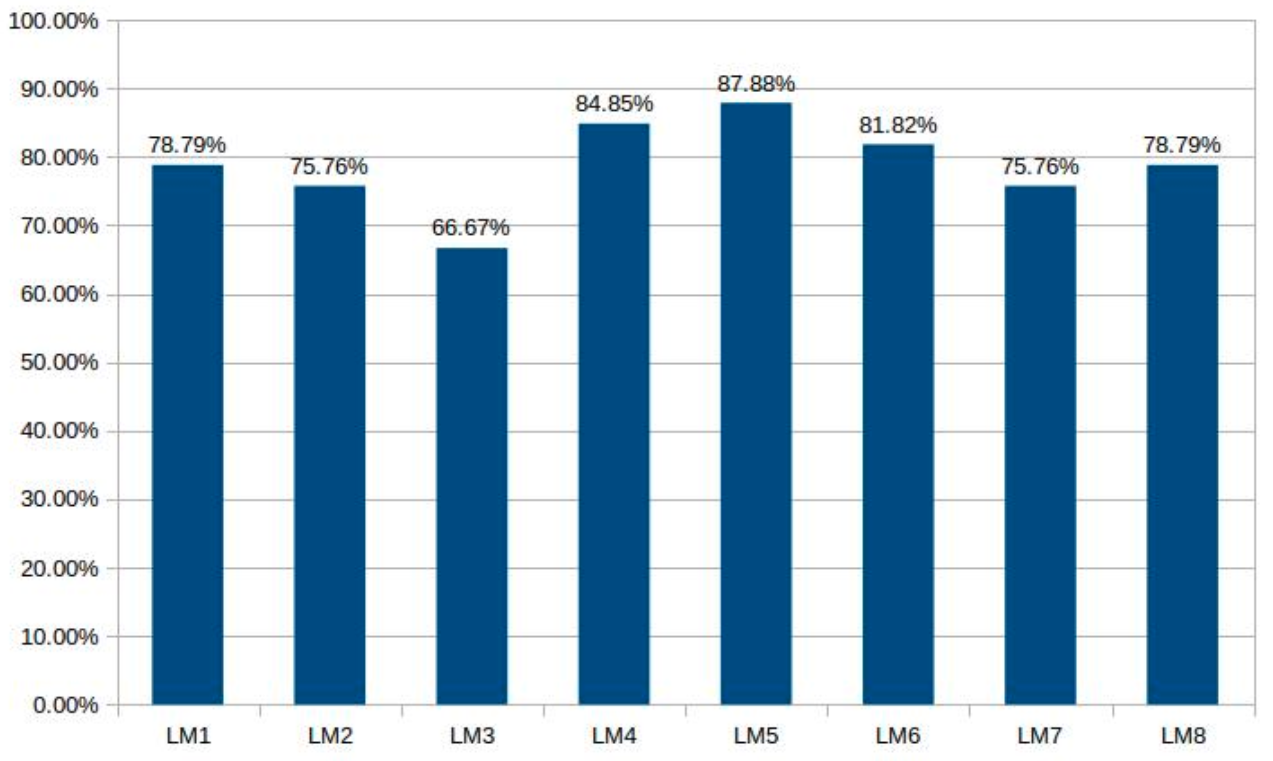
\includegraphics[scale=0.2]{images/chart}}
	\caption{The proportion of acceptable predicted landmarks}
	\label{figchart}
\end{figure}

As a result, the network is able to predict the landmarks on a test set of pronotum images. At statistic side, the predicted landmarks are acceptable. But in image processing side, we expect more about the accuracy (coordinates of predicted landmarks), and the result of CNN is still needed to improve. However, improving on all landmarks is difficult to perform because a number of landmarks have stayed inside the pronotum. Instead of, we will improve the result of the landmarks that stay in the shape of the pronotum.
\section{Improving the predicted landmarks}
\label{secimproving}
In the previous section, we have applied a CNN to predict the landmarks on pronotum images. The results of experiments have shown that the network has worked well to detect the landmarks on the images in the test set. However, when we consider the predicted landmarks by displaying the landmarks on the images, the result is still not precise, specifically, the landmarks stayed on the shape border and at the corner of pronotum. In this section, we describe a scenario to improve the locations of the predicted landmarks which stay at the corner of the pronotum shape, \textit{i.e}  $3^{rd} $ and $7^{th}$ landmarks, called \textit{corner landmarks}. Fig.\ref{figshape} shows the simulation of a pronotum with its shape and manual landmarks. Fig.\ref{figsub11} shows the shape of pronotum and its manual landmarks. The red points represent for the corner landmarks, the yellow points represent the landmarks inside the pronotum. Fig.\ref{figsub22} display an overlap between the shape and real image.

\begin{figure}[htbp]
    \centering
    \begin{subfigure}[t]{0.25\textwidth}
        \centering
        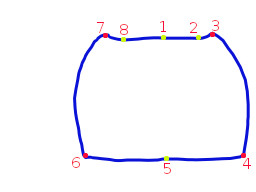
\includegraphics[height=1in]{images/pronotum_model}
        \caption{Pronotum shape with manual landmarks}
        \label{figsub11}
    \end{subfigure}%
    ~ 
    \begin{subfigure}[t]{0.25\textwidth}
        \centering
        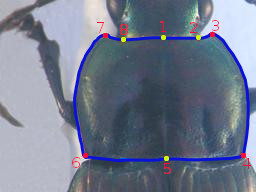
\includegraphics[height=1in]{images/pronotum_overlap}
        \caption{Overlap the pronotum shape and real image}
        \label{figsub22}
    \end{subfigure}
    \caption{The simulator of a pronotum with its shape } 
    \label{figshape}
\end{figure}

\textit{The main idea of this process is generated a general curve through a landmark and tried to adapt the predicted landmark to corresponding general curve,} this work looks like a Procrustes analysis. The scenario starts from the segmentation result of the image. Firstly, from the training dataset, a ``mean curve" is generated for each manual landmark that stays in the shape of pronotum (i.e $3^{rd}, 7^{th}$). Secondly, for each predicted landmark from CNN, we try to adapt the landmark to the contour of pronotum. Finally, we search a pixel around ``adapted point" that the curve via it is closest to the ``mean curve".

\subsection{Generating mean curve}
The mean curve was generated from a set of training images with their manual landmarks. For each image and its manual landmarks, the process to extract the curve via a manual landmark in an image as following:
\begin{enumerate}[nosep]
	\item Segmenting the image to obtain the contour (see \cite{le2017maelab}),
	\item Extracting a patch with the size of $7 \times 7$ centering at the manual landmark\footnote{The size of patch was chosen by experiments.},
	\item Detecting the contour points inside the patch.
\end{enumerate}
The mean curve has obtained by calculating the mean coordinates of points of curves via the manual landmarks that have the same order (same position).

Fig.\ref{figshapect} shows the patch where contains the mean curve through the $3^{rd}$ and the $7^{th}$ landmarks. In the images, the \textit{1-positions} and \textit{0-positions} represent for the pixels belongs to the mean curves (red lines) and not, respectively.

\begin{figure}[htbp]
    \centering
    \begin{subfigure}[t]{0.25\textwidth}
        \centering
        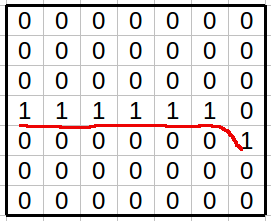
\includegraphics[height=1.35in]{images/curve_lm32}
        \caption{The $3^{rd}$ landmark}
        \label{figsub111}
    \end{subfigure}~
    \begin{subfigure}[t]{0.25\textwidth}
        \centering
        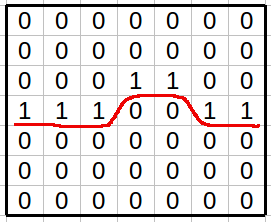
\includegraphics[height=1.35in]{images/curve_lm72}
        \caption{The $7^{th}$ landmark}
        \label{figsub221}
    \end{subfigure}
    \caption{The patches contain mean curves through the manual landmarks } 
    \label{figshapect}
\end{figure}
\subsection{Adapting and improving the predicted landmark}
The predicted landmark (corner landmark) closed to the pronotum but it did not mostly stay on the curve while most of the manual landmark has stayed on the border of pronotum. Therefore, before improving the position of predicted landmark, we need to adapt the landmark on the curve. This process was finished in a simple way that we find the point on the curve that nearest with the predicted landmark.

After finding the point on contour to replace the predicted landmarks. A patch $P_l$ with the size of $15 \times 15$ is created centering at this point. For each contour point in patch $P_l$, a small patch $P_s$ of size $7 \times 7$ is extracted (this patch has the same size with the patch that contains the mean curve). Then, the curve belongs to $P_s$ was detected and compared to the mean curve. The process has been repeated until all contour points of $P_l$ are considered. The point that has the minimum distance with the mean curve will be kept and it was the new coordinates of predicted landmarks.
\subsection{Results}
The proposed scenario has experimented on the $3^{rd}$ and the $7^{th}$ landmarks. For each landmark, the mean curve has been generated from data training images and their manual landmarks. During improving the coordinates of predicted landmarks, Root Mean Square Distance (RMSD) is used to compute the distance between a candiate curve and mean curve. 
Table.\ref{tabledistance2} shows the average error distance of each landmark after improving. \textit{The first column} presents for the order of landmarks; \textit{the second column} presents for the average error distance from CNN result (Table \ref{tabledistance}); \textit{the third column} presents for the average error distance after we improve the coordinates of predicted landmarks. Clearly that, the coordinates of predicted landmarks have been significantly improved ( $33.84\%$ for $3^{rd}$ landmark and $26.3\%$ for $7^{th}$ landmark).

\begin{table}[htbp]
\centering
\begin{tabular}{c|p{1.5cm}|p{1.5cm}}

\textbf{$\#$Landmark} & \textbf{CNN} & \textbf{Improved} \\ \hline
$3^{rd}$ & 4.2959 & \textbf{2.8421}  \\ \hline
$7^{th}$ & 4.6360 & \textbf{3.4166} \\ 
\end{tabular}
\caption{A comparison of the average error distances on each landmark }
\label{tabledistance2}
\end{table}

In another side, we would like take into account the number of acceptable landmarks by applying the same way than we have done with CNN (standard deviation). Fig.\ref{figchart2} shows a comparison of the proportions of acceptable per landmark (in percent) between two periods (before and after improving the coordinates of predicted landmarks). According to the figure, the proportion of acceptable on $3^{rd}$ landmark has improved around $23.09\%$, while this rate at $7^{th}$ landmark is $15.02\%$. Comparing with the output from CNN, the coordinates of predicted landmarks at position $3$ and $7$ have been vastly improved.

\begin{figure}[htbp]
	\centerline{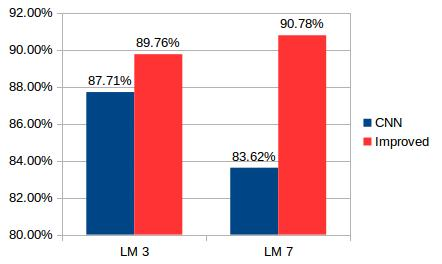
\includegraphics[scale=0.8]{images/chart_cnn_improving}}
	\caption{A comparison of the proportions of acceptable predicted landmarks on $3^{rd}$ and $7^{th}$ landmarks. The \textit{blue} and \textit{red} columns present for the ratio of accuracy of predicted landmarks which given by CNN and improving method, respectively.}
	\label{figchart2}
\end{figure}

As a result of working, the program outputs the
predicted-landmarks of the images as TPS files. With the outputs are TPS files,
the user can use MAELab framework\footnote{MAELab is a free software written in C++. It can be directly and freely
obtained by request at the authors.} to display the
landmarks on the images.
\section{Conclusions}
In this paper, we have presented a scenario to predict the landmark on beetle's head images. It includes two steps: predicting and improving the coordinates of estimated landmarks. 

The prediction step has been done by applying deep learning. A CNN has been designed with three times repeated structure which consists of a convolutional layer, a max pooling layer, and a dropout layer, followed by the connected layers. During the training phase, the CNN have been trained with several times in different selections of training data. After training, the network was able to predict the landmarks on the images in the test set. The result has been evaluated by comparing the coordinates between predicted and manual landmarks. The quality of prediction allows using automatic
landmarking to replace manual landmarks in some aspects. However, we expect more accuracy on the landmarks belongs to the contour of the images, and they have been improved.

The improvement of predicted landmarks has finished as a technique of Procrustes analysis. From the training dataset and their manual landmarks, the mean curves through the landmarks in the contours have been generated. Then, the predicted landmarks by CNN have been adapted and improved. The results have shown that using the convolutional network to predict the landmarks on biological images is promising good results in the case that the image was difficult to segment. But with a limited number of data, we need to improve the result by another method. Therefore, future research in landmarking identification appears as an improved of the worth exploring.

\section*{Acknowledgements}
The research has been supported by INRA. We would like to thank the biologists, who have provided the dataset. We thank also our colleague, Nicolas PARISEY, who provided insight and expertise that greatly assisted the research.

\bibliography{IEEEabrv,includes/icdp2009}


\end{document}
